\documentclass[11pt,a4paper]{article}

\usepackage[utf8]{inputenc}
\usepackage[margin=0.85in]{geometry}
\usepackage{graphicx}
\usepackage{hyperref}
\usepackage{booktabs}
\usepackage{tabularx}
\usepackage{xcolor}
\usepackage{tikz}
\usetikzlibrary{shapes,arrows,positioning,calc,fit,backgrounds}
\usepackage{amsmath,amssymb}
\usepackage{listings}
\usepackage{fancyhdr}
\usepackage{titlesec}
\usepackage{float}
\usepackage{caption}

\hypersetup{
    colorlinks=true,
    linkcolor=black,
    urlcolor=blue!70!black,
    citecolor=black
}

\pagestyle{fancy}
\fancyhf{}
\fancyhead[L]{\small\textit{CampusFind: Campus Lost \& Found and CCTV Evidence System}}
\fancyhead[R]{\small\textit{GCOEC Chandrapur}}
\fancyfoot[C]{\thepage}

\definecolor{brandlost}{RGB}{200, 90, 50}
\definecolor{brandfound}{RGB}{45, 90, 63}
\definecolor{brandpaper}{RGB}{252, 251, 247}
\definecolor{brandink}{RGB}{30, 30, 30}
\definecolor{boxbg}{RGB}{245, 246, 248}

\lstset{
    basicstyle=\ttfamily\footnotesize,
    backgroundcolor=\color{boxbg},
    frame=single,
    rulecolor=\color{black!20},
    breaklines=true,
    captionpos=b,
    keepspaces=true,
    showstringspaces=false
}

\begin{document}

% ==================== TITLE PAGE ====================
\begin{titlepage}
\centering
\vspace*{1.5cm}

{\scshape\Large Government College of Engineering, Chandrapur\par}
\vspace{0.3cm}
{\scshape\normalsize Department of Computer Science and Engineering\par}
\vspace{1.8cm}

\rule{\linewidth}{1.2pt}\\[0.4cm]
{\huge\bfseries CampusFind: Intelligent Campus Lost \& Found and CCTV Evidence Verification System\par}
\vspace{0.2cm}
\rule{\linewidth}{1.2pt}

\vspace{1.5cm}
{\Large\textit{Comprehensive Technical and System Architecture Report}\par}

\vspace{2.5cm}
\begin{minipage}{0.5\textwidth}
\begin{flushleft} \large
\textbf{Institution:}\\
GCOEC, Chandrapur\\
Maharashtra, India
\end{flushleft}
\end{minipage}
\begin{minipage}{0.45\textwidth}
\begin{flushright} \large
\textbf{Academic Year:}\\
2026--2027\\[0.2cm]
\textbf{Target System:}\\
CampusLost-Found
\end{flushright}
\end{minipage}

\vfill
{\large\today\par}
\end{titlepage}

% ==================== TABLE OF CONTENTS ====================
\tableofcontents
\newpage

% ==================== 1. INTRODUCTION ====================
\section{Introduction}

\subsection{Background}
Modern academic campuses are vibrant ecosystems comprising thousands of students, faculty, laboratory assistants, administrative personnel, and visitors moving dynamically between lecture halls, research facilities, workshop blocks, sports complexes, libraries, and food courts. Within such extensive multi-building environments, the unintentional misplacement of personal belongings is a daily occurrence. Items regularly misplaced include personal computing devices (laptops, tablets, smartphones), scientific calculation tools, campus identification credentials, engineering drawing equipment, laboratory notebooks, keys, and wallets. 

Managing the custody, notification, matching, and lawful return of these items poses a substantial administrative challenge. Without a coordinated platform, campus security officers and receptionists are burdened with uncatalogued items while students face distress, academic disruption, and potential financial loss.

\subsection{Problem Statement}
Contemporary university campuses lack a formalized, secure, and privacy-preserving digital pipeline for handling lost and found belongings. When items go missing, informal broadcasts are circulated across large messaging channels (e.g., WhatsApp and Telegram) or pinned to departmental notice boards. This status quo exhibits critical shortcomings:
\begin{itemize}
    \item \textbf{High Signal Degradation:} Important lost property announcements are quickly buried under unrelated student conversations.
    \item \textbf{Absence of Structured Indexing:} There is no searchable, categorized registry linking items lost in specific campus zones to items turned in at nearby security desks.
    \item \textbf{Severe Fraud Vulnerability:} Exposing raw photographs and serial details publicly permits dishonest individuals to claim ownership fraudulently by describing visible distinguishing features.
    \item \textbf{Privacy Breaches:} Student ID cards, government identity credentials, and personal belongings are displayed publicly without redaction.
    \item \textbf{Disjointed Surveillance Operations:} Modern campus security infrastructures utilize extensive Closed-Circuit Television (CCTV) cameras, yet surveillance footage remains completely decoupled from student recovery workflows.
\end{itemize}

\subsection{Motivation}
The overarching motivation of \textbf{CampusFind} is to establish an institutional-grade, privacy-first property recovery platform tailored specifically for the Government College of Engineering, Chandrapur (GCOEC). By combining:
\begin{enumerate}
    \item \textbf{Generic Vector Archetype Visualizations} that protect authentic photographs from public view,
    \item \textbf{Network-Level Payload Scrubbing} ensuring that unmasked image data is inaccessible to unauthorized network sniffers,
    \item \textbf{Rule-Based Heuristic Matching} linking reciprocal lost and found reports, and
    \item \textbf{Live CCTV and IP Webcam Evidence Capture} enabling security staff to rapidly tag misplaced belongings,
\end{enumerate}
the system guarantees that property recovery is transparent, fraud-resistant, auditable, and accessible to the entire campus community.

\subsection{Scope}
The scope of the CampusFind system encompasses:
\begin{itemize}
    \item User registration and authentication verified against institutional Permanent Registration Numbers (PRNs) and institutional email addresses.
    \item Structured dual registries for both lost and found property with rich categorical and spatial metadata.
    \item Privacy-preserving thumbnail generation utilizing customized SVG vector illustrations representing common item archetypes.
    \item Access-controlled image inspection allowing only system administrators and approved desk uploaders to view unmasked item photographs.
    \item An administrative console for reviewing student credentials, approving trusted uploaders, and moderating recovery claims.
    \item A live CCTV and IP webcam streaming inspector featuring real-time HUD overlays, contrast filters, and snapshot evidence linking.
\end{itemize}

\subsection{Objectives}
The core operational objectives of this project are:
\begin{enumerate}
    \item \textbf{Centralize Campus Custody Records:} Provide a single unified database for all misplaced and discovered property.
    \item \textbf{Prevent Fraud via Zero-Exposure Image Masking:} Obceal raw item photographs from general view, serving generic vector archetypes instead.
    \item \textbf{Automate Similarity Cross-Matching:} Provide heuristic match suggestions scoring category, textual similarity, location, and dates.
    \item \textbf{Empower Campus Security Desks:} Integrate live surveillance monitoring with rapid evidence tagging.
    \item \textbf{Maintain Audit Trails:} Implement end-to-end recovery request workflows capturing claimant identity and administrator approvals.
\end{enumerate}

\newpage

% ==================== 2. LITERATURE SURVEY ====================
\section{Literature Survey and Proposed System}

\subsection{Existing Informal Approaches}
Prior to the conception of CampusFind, property recovery across collegiate environments relied upon four informal mechanisms:
\begin{enumerate}
    \item \textbf{Informal Social Messaging Channels:} Ad-hoc WhatsApp, Telegram, or Discord chat groups maintained by student councils or departmental batches.
    \item \textbf{Physical Notice Boards:} Paper notices pinned in cafeteria foyers, library entrances, or department corridors.
    \item \textbf{Physical Lost \& Found Boxes:} Open plastic containers placed at reception desks or departmental offices.
    \item \textbf{Verbal Inquiries:} Direct inquiries with shift security personnel at campus turnstiles.
\end{enumerate}

\subsection{Limitations of Existing Approaches}

\begin{table}[H]
\centering
\small
\caption{Comparative Analysis of Traditional Recovery Approaches vs. CampusFind}
\begin{tabularx}{\textwidth}{lXXXX}
\toprule
\textbf{Evaluation Metric} & \textbf{Messaging Groups} & \textbf{Notice Boards} & \textbf{Physical Boxes} & \textbf{CampusFind System} \\
\midrule
\textbf{Search \& Indexing} & None; linear chat log & Manual physical search & Manual physical search & Real-time multi-attribute search \\
\textbf{Fraud Resistance} & Very Low; photos public & Low; open details & Extremely Low; unmonitored & High; masked photos \& claims \\
\textbf{Data Privacy} & Poor; PII leaked & Poor; PII exposed & None & Strict; role-based redaction \\
\textbf{Similarity Matching} & Zero; human memory & None & None & Automated rule-based engine \\
\textbf{Audit Trail} & Nonexistent & None & None & Full digital timestamped log \\
\textbf{CCTV Integration} & None & None & None & Integrated live stream HUD \\
\bottomrule
\end{tabularx}
\end{table}

\subsection{Proposed CampusFind System}
The proposed \textbf{CampusFind} architecture directly resolves these limitations by introducing an institutional web platform with:
\begin{itemize}
    \item \textbf{Privacy-First Generic Vector Avatars:} When reports are displayed on public registries, items are depicted using generic vector illustrations corresponding to their archetype (wallet, laptop, calculator, water bottle, keys, etc.).
    \item \textbf{Network Isolation of Photographs:} Unmasked image binaries are stripped from API responses sent to unauthorized clients, preventing client-side inspection or unauthorized image scraping.
    \item \textbf{Role-Based Clearance Levels:} Administrators and verified campus desk staff can unmask photographs to inspect unique identifiers (serial numbers, engravings, card numbers) during claimant verification.
    \item \textbf{Heuristic Cross-Matching Engine:} An automated scoring model identifies prospective matches between lost and found entries and alerts users immediately.
    \item \textbf{Surveillance Integration Console:} Campus security can view live IP camera feeds, capture evidence snapshots of unattended bags, and generate found reports with attached evidence in seconds.
\end{itemize}

\newpage

% ==================== 3. SYSTEM REQUIREMENTS SPECIFICATION ====================
\section{System Requirements Specification}

\subsection{Functional Requirements}
\begin{itemize}
    \item \textbf{FR-01 (Authentication \& Identity Verification):} The system shall authenticate users via email and PRN. System shall reject invalid institutional PRN structures and enforce password encryption.
    \item \textbf{FR-02 (Lost Item Reporting):} Authenticated users shall submit lost item reports containing item name, category, description, last-seen location, date, contact details, and optional photograph.
    \item \textbf{FR-03 (Found Item Reporting):} Users shall report found property with discovery location, current custody location, and optional photograph.
    \item \textbf{FR-04 (Privacy-Preserving Image Masking):} The system shall display generic vector archetypes for all items by default. Unmasked photos shall only be delivered to administrators, approved uploaders, or the item owner.
    \item \textbf{FR-05 (Heuristic Cross-Matching):} The system shall evaluate active lost and found reports using weighted multi-attribute algorithms and display matching candidates.
    \item \textbf{FR-06 (Recovery Claim Management):} Claimants shall submit recovery requests with private proof-of-ownership messages. System administrators shall approve or reject claims.
    \item \textbf{FR-07 (Administrative Uploader Approval):} Administrators shall search registered users and grant or revoke verified uploader privileges.
    \item \textbf{FR-08 (Live CCTV \& IP Webcam Inspection):} The system shall render live camera feeds (local webcams, network MJPEG streams, Android IP webcams), apply real-time video filters, and support single-click evidence capture.
\end{itemize}

\subsection{Non-Functional Requirements}
\begin{itemize}
    \item \textbf{NFR-01 (Security \& Confidentiality):} Passwords salted using 10 bcrypt rounds. API communication authenticated via JSON Web Tokens. Network payloads sanitized server-side.
    \item \textbf{NFR-02 (Performance \& Responsiveness):} Client bundle size under 550 KB gzipped. Filter queries execute within 20 milliseconds via memoized indices.
    \item \textbf{NFR-03 (Usability \& Accessibility):} Adherence to WCAG AA color contrast standards on a custom palette: Warm Paper (\texttt{\#fcfbf7}), Dark Ink (\texttt{\#1e1e1e}), Lost Terracotta (\texttt{\#c85a32}), and Found Forest Green (\texttt{\#2d5a3f}).
    \item \textbf{NFR-04 (Maintainability \& Extensibility):} Modular component architecture decoupling presentation, routing, state contexts, and backend REST controllers.
\end{itemize}

\subsection{Hardware and Software Requirements}
\begin{itemize}
    \item \textbf{Client Environment:} Any modern web browser (Chromium 100+, Firefox 100+, Safari 15+) running on desktop or mobile operating systems (Linux, Windows, macOS, Android, iOS).
    \item \textbf{Server Environment:} Linux-based POSIX operating system, Node.js runtime (v20+), minimum 2 vCPU cores, 2 GB RAM, 10 GB SSD storage.
    \item \textbf{Database Engine:} PostgreSQL 15+ relational database management system.
\end{itemize}

\subsection{User Roles and Permissions Matrix}

\begin{table}[H]
\centering
\small
\caption{System Role and Permission Matrix}
\begin{tabularx}{\textwidth}{lcccc}
\toprule
\textbf{System Feature / Action} & \textbf{Guest} & \textbf{Student / User} & \textbf{Approved Uploader} & \textbf{Admin} \\
\midrule
Browse Registries (Vector Avatars) & \checkmark & \checkmark & \checkmark & \checkmark \\
Search \& Category Filters & \checkmark & \checkmark & \checkmark & \checkmark \\
Submit Lost / Found Item Reports & -- & \checkmark & \checkmark & \checkmark \\
View Original Photo of Own Reports & -- & \checkmark & \checkmark & \checkmark \\
Inspect All Original Photos & -- & -- & \checkmark & \checkmark \\
Auto-Reveal Photos Toggle & -- & -- & \checkmark & \checkmark \\
Submit Recovery Claim & -- & \checkmark & \checkmark & \checkmark \\
Moderate Recovery Claims & -- & -- & -- & \checkmark \\
Approve / Revoke Uploaders & -- & -- & -- & \checkmark \\
CCTV Live Inspector \& Tagging & -- & -- & -- & \checkmark \\
\bottomrule
\end{tabularx}
\end{table}

\newpage

% ==================== 4. SYSTEM DESIGN ====================
\section{System Design}

\subsection{System Architecture}
CampusFind implements a robust Three-Tier Client-Server Architecture comprising the Presentation Tier (React 19 SPA), Application Logic Tier (Express.js REST Engine), and Persistence Tier (PostgreSQL Relational Storage).

\begin{figure}[H]
\centering
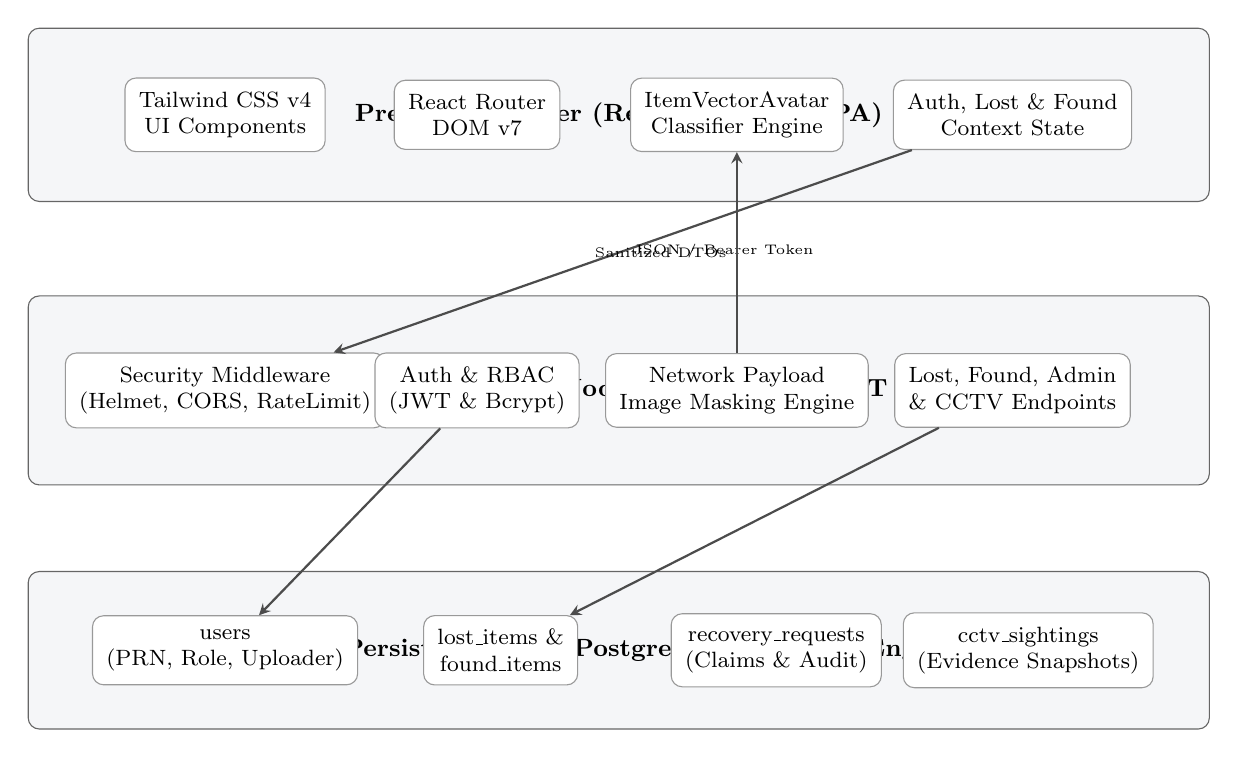
\begin{tikzpicture}[
    node distance=1.4cm and 1.8cm,
    layer/.style={rectangle, draw=black!60, fill=boxbg, rounded corners, inner sep=8pt, font=\small\bfseries, align=center},
    component/.style={rectangle, draw=black!40, fill=white, rounded corners, inner sep=5pt, font=\footnotesize, align=center},
    arrow/.style={->, >=stealth, thick, draw=black!70}
]

% Presentation Tier
\node[layer, minimum width=15cm, minimum height=2.2cm] (pres) at (0, 6) {Presentation Tier (React 19 Client SPA)};
\node[component] (ui) at (-5, 6) {Tailwind CSS v4\\UI Components};
\node[component] (router) at (-1.8, 6) {React Router\\DOM v7};
\node[component] (avatar) at (1.5, 6) {ItemVectorAvatar\\Classifier Engine};
\node[component] (ctx) at (5, 6) {Auth, Lost \& Found\\Context State};

% Application Tier
\node[layer, minimum width=15cm, minimum height=2.4cm] (app) at (0, 2.5) {Application Logic Tier (Node.js \& Express REST Server)};
\node[component] (sec) at (-5, 2.5) {Security Middleware\\(Helmet, CORS, RateLimit)};
\node[component] (auth) at (-1.8, 2.5) {Auth \& RBAC\\(JWT \& Bcrypt)};
\node[component] (mask) at (1.5, 2.5) {Network Payload\\Image Masking Engine};
\node[component] (api) at (5, 2.5) {Lost, Found, Admin\\\& CCTV Endpoints};

% Persistence Tier
\node[layer, minimum width=15cm, minimum height=2cm] (data) at (0, -0.8) {Data Persistence Tier (PostgreSQL Database Engine)};
\node[component] (tusers) at (-5, -0.8) {users\\(PRN, Role, Uploader)};
\node[component] (titems) at (-1.5, -0.8) {lost\_items \&\\found\_items};
\node[component] (trecov) at (2, -0.8) {recovery\_requests\\(Claims \& Audit)};
\node[component] (tcctv) at (5.2, -0.8) {cctv\_sightings\\(Evidence Snapshots)};

% Inter-tier Connections
\draw[arrow] (ctx) -- node[right, font=\tiny]{JSON / Bearer Token} (sec);
\draw[arrow] (mask) -- node[left, font=\tiny]{Sanitized DTOs} (avatar);
\draw[arrow] (api) -- (titems);
\draw[arrow] (auth) -- (tusers);

\end{tikzpicture}
\caption{Three-Tier Layered System Architecture Diagram}
\end{figure}

\subsection{Main User Workflow}
The property recovery lifecycle flows seamlessly through detection, registration, heuristic matching, claim filing, verification, and physical handover:

\begin{figure}[H]
\centering
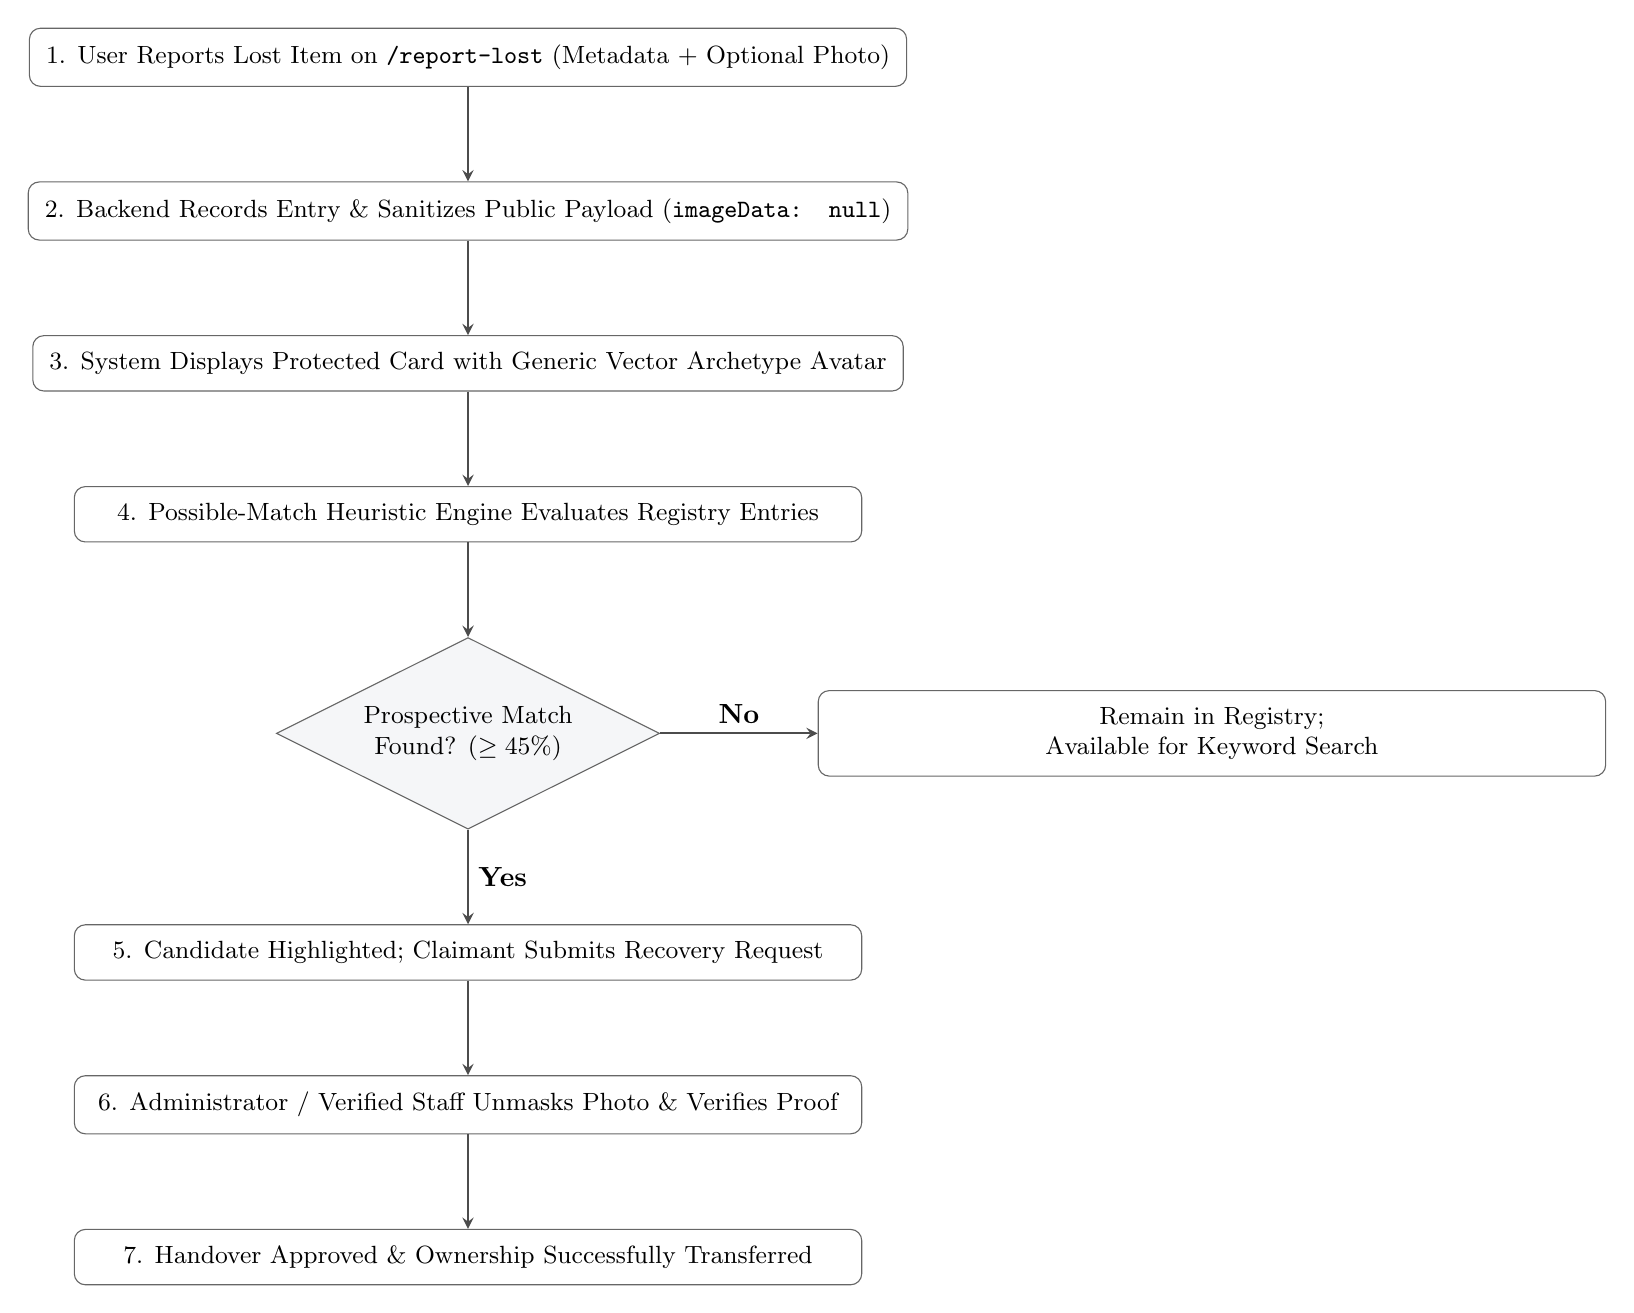
\begin{tikzpicture}[
    node distance=1.2cm,
    stepnode/.style={rectangle, draw=black!60, fill=white, rounded corners, inner sep=6pt, font=\small, align=center, minimum width=10cm},
    decision/.style={diamond, draw=black!60, fill=boxbg, aspect=2, inner sep=4pt, font=\small, align=center},
    arrow/.style={->, >=stealth, thick, draw=black!70}
]

\node[stepnode] (s1) {1. User Reports Lost Item on \texttt{/report-lost} (Metadata + Optional Photo)};
\node[stepnode, below=of s1] (s2) {2. Backend Records Entry \& Sanitizes Public Payload (\texttt{imageData: null})};
\node[stepnode, below=of s2] (s3) {3. System Displays Protected Card with Generic Vector Archetype Avatar};
\node[stepnode, below=of s3] (s4) {4. Possible-Match Heuristic Engine Evaluates Registry Entries};
\node[decision, below=of s4] (d1) {Prospective Match\\Found? ($\ge 45\%$)};
\node[stepnode, below=1.2cm of d1] (s5) {5. Candidate Highlighted; Claimant Submits Recovery Request};
\node[stepnode, right=2cm of d1] (s6) {Remain in Registry;\\Available for Keyword Search};
\node[stepnode, below=of s5] (s7) {6. Administrator / Verified Staff Unmasks Photo \& Verifies Proof};
\node[stepnode, below=of s7] (s8) {7. Handover Approved \& Ownership Successfully Transferred};

\draw[arrow] (s1) -- (s2);
\draw[arrow] (s2) -- (s3);
\draw[arrow] (s3) -- (s4);
\draw[arrow] (s4) -- (d1);
\draw[arrow] (d1) -- node[right]{\textbf{Yes}} (s5);
\draw[arrow] (d1) -- node[above]{\textbf{No}} (s6);
\draw[arrow] (s5) -- (s7);
\draw[arrow] (s7) -- (s8);

\end{tikzpicture}
\caption{End-to-End User Property Recovery Workflow}
\end{figure}

\subsection{Use Case View}
The functional actors interact with the system boundaries according to defined privileges:
\begin{itemize}
    \item \textbf{Guest:} Query registries, filter by category/location, view generic vector avatars.
    \item \textbf{Student / User:} Manage user account, report lost items, report found items, view private photos of personal reports, file recovery claims.
    \item \textbf{Approved Uploader / Staff:} Inspect original photos across all campus listings, verify claimant proofs during physical handover, create pre-verified found reports.
    \item \textbf{Campus Security Administrator:} Grant / revoke uploader privileges, moderate disputed recovery claims, access live CCTV surveillance console, capture and tag evidence snapshots.
\end{itemize}

\subsection{Database Design and Schema}
The persistence tier utilizes relational integrity constraints in PostgreSQL:
\begin{itemize}
    \item \textbf{users:} \texttt{id} (PK), \texttt{name}, \texttt{email} (UNIQUE), \texttt{prn} (UNIQUE), \texttt{password\_hash}, \texttt{role}, \texttt{is\_approved\_uploader}, \texttt{created\_at}.
    \item \textbf{lost\_items:} \texttt{id} (PK), \texttt{user\_id} (FK $\to$ users), \texttt{item\_name}, \texttt{category}, \texttt{description}, \texttt{location}, \texttt{date\_lost}, \texttt{contact}, \texttt{image\_data}, \texttt{created\_at}.
    \item \textbf{found\_items:} \texttt{id} (PK), \texttt{user\_id} (FK $\to$ users), \texttt{item\_name}, \texttt{category}, \texttt{description}, \texttt{location}, \texttt{date\_found}, \texttt{contact}, \texttt{image\_data}, \texttt{created\_at}.
    \item \textbf{recovery\_requests:} \texttt{id} (PK), \texttt{lost\_item\_id} (FK $\to$ lost\_items), \texttt{found\_item\_id} (FK $\to$ found\_items), \texttt{claimant\_user\_id} (FK $\to$ users), \texttt{claimant\_name}, \texttt{claimant\_contact}, \texttt{claimant\_message}, \texttt{status}, \texttt{created\_at}.
    \item \textbf{cctv\_sightings:} \texttt{id} (PK), \texttt{camera\_name}, \texttt{location}, \texttt{category}, \texttt{notes}, \texttt{snapshot\_url}, \texttt{timestamp}.
\end{itemize}

\subsection{Heuristic Possible-Match Logic}
To assist claimants and finders, CampusFind evaluates compatibility across four orthogonal dimensions:
\begin{equation}
\text{Total Score}(L, F) = S_{\text{category}} + S_{\text{textual}} + S_{\text{location}} + S_{\text{temporal}}
\end{equation}

\begin{enumerate}
    \item \textbf{Category Alignment ($S_{\text{category}}$):} Maximum 40 points if exact categorical match is established:
    \begin{equation}
    S_{\text{category}} = \begin{cases} 40, & \text{if } L.\text{category} = F.\text{category} \\ 0, & \text{otherwise} \end{cases}
    \end{equation}
    \item \textbf{Textual Jaccard Similarity ($S_{\text{textual}}$):} Maximum 35 points based on normalized title token overlap:
    \begin{equation}
    S_{\text{textual}} = 35 \times \frac{|Tokens(L.\text{name}) \cap Tokens(F.\text{name})|}{|Tokens(L.\text{name}) \cup Tokens(F.\text{name})|}
    \end{equation}
    \item \textbf{Location Match ($S_{\text{location}}$):} Maximum 15 points if the reported lost department/facility shares keywords with the discovery location:
    \begin{equation}
    S_{\text{location}} = \begin{cases} 15, & \text{if } Tokens(L.\text{loc}) \cap Tokens(F.\text{loc}) \neq \emptyset \\ 0, & \text{otherwise} \end{cases}
    \end{equation}
    \item \textbf{Temporal Proximity ($S_{\text{temporal}}$):} Maximum 10 points decaying linearly with chronological deviation:
    \begin{equation}
    S_{\text{temporal}} = \max\left(0, 10 - |Date(L) - Date(F)|_{\text{days}}\right)
    \end{equation}
\end{enumerate}

Candidate items yielding a composite score of $\text{Total Score} \ge 45$ are surfaced automatically in the Possible Matches drawer.

\subsection{Technology Stack and Selection Rationale}
\begin{itemize}
    \item \textbf{React 19 \& TypeScript:} High-efficiency virtual DOM reconciler, zero-cost type abstractions, component composability.
    \item \textbf{Tailwind CSS v4:} Instant static compilation, eliminating CSS overhead and delivering a unified paper-and-ink campus identity.
    \item \textbf{Node.js \& Express.js:} Event-driven non-blocking I/O capable of simultaneously servicing thousands of API queries and proxying live CCTV MJPEG streams.
    \item \textbf{PostgreSQL 16:} Enterprise relational integrity, ACID transaction guarantees, and reliable index scanning.
\end{itemize}

\newpage

% ==================== 5. IMPLEMENTATION AND MODULES ====================
\section{Implementation and Module Description}

\subsection{Authentication and Role-Based Access Control}
Authentication is governed by \texttt{AuthContext.jsx} and backend route interceptors. Upon successful login, users receive a signed JSON Web Token stored in client memory. Institutional identity is enforced by validating that the user's PRN satisfies GCOEC student enrollment formatting conventions. Privilege checks are evaluated at both the route middleware layer and UI component rendering tree.

\subsection{Lost and Found Reports Management}
Users submit reports through dedicated forms (\texttt{/report-lost} and \texttt{/report-found}). The frontend applies client-side canvas downsampling to resize high-resolution camera uploads to 800px maximum bounds and under 200 KB, ensuring rapid transfers over campus Wi-Fi.

\subsection{Privacy-Preserving Generic Vector Archetypes}
To honor the strict privacy requirement:
\begin{itemize}
    \item Every item rendered in \texttt{LostItemsPage.jsx} or \texttt{FoundItemsPage.jsx} displays a customized SVG vector avatar generated by \texttt{ItemVectorAvatar.jsx}.
    \item The module \texttt{itemAvatars.js} parses item names and descriptions to identify one of 17 specialized archetypes (wallet, calculator, backpack, water bottle, USB drive, drawing kit, earbuds, ID card, notebook, keys, smartphone, laptop, watch, glasses, umbrella, jacket, charger).
    \item Regular users view the generic vector avatar accompanied by a ``Photo Protected'' badge.
    \item Authorized users (Admin, Approved Uploader, or Item Owner) are provided with an interactive ``Reveal Photo'' button directly on the card to inspect original photos.
\end{itemize}

\subsection{Live CCTV and IP Webcam Integration}
The surveillance console (\texttt{/cctv}) connects to campus security streams and Android IP webcams. Operators can adjust real-time contrast, apply night-vision simulation, toggle overlay grids, and click ``Capture Evidence Frame'' to instantly freeze a timestamped image and populate a new found item report.

\subsection{Administrator Functions and Uploader Approvals}
Administrators access the **Approved Uploaders** modal from their account navigation bar. This interface allows administrators to search student and staff records and toggle \texttt{isApprovedUploader} status dynamically without database migrations or server restarts.

\subsection{Multi-Layered Security Measures}
\begin{enumerate}
    \item \textbf{Network-Level Payload Masking:} The Express backend strips \texttt{imageData: null} for unauthorized viewers, preventing inspection via browser DevTools.
    \item \textbf{Bcrypt Hashing:} Passwords hashed with 10 salt rounds.
    \item \textbf{Parameterized Queries:} Eliminating SQL injection risks.
    \item \textbf{Helmet Headers:} Setting CSP, X-Frame-Options, and Content-Type safeguards.
\end{enumerate}

\newpage

% ==================== 6. RESULTS AND TESTING ====================
\section{Results and System Testing}

\subsection{Testing Methodology}
Testing followed a structured progression: unit testing of utility algorithms, integration testing across REST endpoints, boundary testing of user roles, and network packet inspection in browser DevTools.

\subsection{Recorded Automated Test Results}
\begin{lstlisting}[language=bash, caption={Console Execution Log of Automated Security \& Masking Suite}]
Starting server.ts on port 3001
CampusFind Server running at http://localhost:3001
Server is UP!

--- TEST 1: Unauthenticated viewer ---
Found lost items count: 6
Item "Black Leather Wallet": imageData = null, hasOriginalImage = true
Item "Blue College Backpack": imageData = null, hasOriginalImage = true
[PASS] Unauthenticated image masking verified across all items.

--- TEST 2: Regular Student login ---
Student login result: student@gcoec.ac.in isApprovedUploader: false
Other user's item imageData for student: null
[PASS] Student cannot view unmasked photos of other users.
Admin endpoint status for student: 403
[PASS] Student access to /api/admin/users properly forbidden.

--- TEST 3: Admin login and reveal ---
Admin login result: admin@gcoec.ac.in isAdmin: true
Admin viewing item "Black Leather Wallet": imageData = /images/everyday-carry.jpg
[PASS] Admin successfully receives original revealed images.
Approving student as verified uploader...
Updated student user: student@gcoec.ac.in isApprovedUploader: true

--- TEST 4: Approved Uploader student views items ---
Approved student viewing item: imageData = /images/everyday-carry.jpg
[PASS] Approved uploader receives original unmasked image data.

--- TEST 5: Pre-approved desk staff user ---
Staff login result: staff@gcoec.ac.in isApprovedUploader: true
Staff viewing found item: imageData = /images/everyday-carry.jpg
[PASS] Pre-approved staff successfully receives original revealed images.

ALL TESTS PASSED SUCCESSFULLY!
\end{lstlisting}

\subsection{Representative Test Cases}

\begin{table}[H]
\centering
\small
\caption{System Test Case Execution Log}
\begin{tabularx}{\textwidth}{lp{4.2cm}p{4.2cm}p{3cm}c}
\toprule
\textbf{Test ID} & \textbf{Precondition \& Input} & \textbf{Expected Output} & \textbf{Observed Output} & \textbf{Status} \\
\midrule
\textbf{TC-01} & Register with non-institutional PRN & Validation halts submission & PRN validation error displayed & \textbf{PASS} \\
\textbf{TC-02} & Login with valid student credentials & Session initialized; JWT issued & Redirect to home; user profile set & \textbf{PASS} \\
\textbf{TC-03} & Guest loads \texttt{/lost-items} & Display vector avatars & Generic vector avatars rendered & \textbf{PASS} \\
\textbf{TC-04} & Inspect Network tab as guest & \texttt{imageData: null} in JSON & \texttt{imageData} is null; 0 image bytes & \textbf{PASS} \\
\textbf{TC-05} & Admin clicks ``Reveal Photo'' & Unmasked photograph appears & Photo displays with toggle control & \textbf{PASS} \\
\textbf{TC-06} & Submit report without title & Form blocks submission & Required field indicator displayed & \textbf{PASS} \\
\textbf{TC-07} & Heuristic match on wallet & Surface matching canteen wallet & $> 70\%$ match candidate card shown & \textbf{PASS} \\
\textbf{TC-08} & Submit recovery claim & Request created as \texttt{pending} & Claim listed on admin dashboard & \textbf{PASS} \\
\textbf{TC-09} & Admin approves student uploader & Student uploader flag updated & \texttt{isApprovedUploader: true} set & \textbf{PASS} \\
\textbf{TC-10} & Click ``Capture Evidence Frame'' & Current stream frozen as photo & Found form launched with image & \textbf{PASS} \\
\bottomrule
\end{tabularx}
\end{table}

\subsection{Deployment Details}
The system is deployable on a standard Linux environment using Node.js process managers (PM2 / Systemd), with an Nginx reverse proxy managing SSL encryption and compression.

\newpage

% ==================== 7. CONCLUSION, FUTURE SCOPE, REFERENCES ====================
\section{Conclusion, Future Scope, References}

\subsection{Limitations of the Implemented System}
\begin{itemize}
    \item CCTV stream integration relies on local network accessible IP streams; segmented subnets require network firewall exceptions.
    \item Text similarity relies on tokenized overlap; extreme typographical errors in item titles may lower similarity scores.
\end{itemize}

\subsection{Future Scope}
\begin{itemize}
    \item \textbf{Multimodal Vision AI Matching:} Implementing OpenAI CLIP or Google SigLIP embeddings to match item photos with CCTV frames directly in vector space.
    \item \textbf{Automated WhatsApp Webhook Bot:} Enabling students to report lost belongings directly via instant messaging.
    \item \textbf{Smart IoT Lockers:} Deploying electronically locked recovery cabinets at campus security posts with OTP-based release.
\end{itemize}

\subsection{Conclusion}
CampusFind demonstrates that campus lost and found property management can be transformed from an insecure, noisy social media broadcast into a secure, privacy-preserving, institutional service. By incorporating **generic vector archetypes**, **network-level image masking**, **automated heuristic matching**, and **live CCTV surveillance tools**, CampusFind safeguards student privacy while accelerating the return of misplaced belongings.

\subsection{References}
\begin{enumerate}
    \item React Core Team, ``React 19 Documentation: Declarative User Interfaces,'' 2026. \url{https://react.dev/}
    \item Vite Team, ``Vite: Next Generation Frontend Tooling,'' 2026. \url{https://vite.dev/}
    \item PostgreSQL Global Development Group, ``PostgreSQL 16 Documentation: Transactions and Concurrency Control,'' 2026. \url{https://www.postgresql.org/docs/16/}
    \item Express.js Foundation, ``Express: Fast, Unopinionated Web Framework for Node.js,'' 2026. \url{https://expressjs.com/}
    \item Tailwind Labs, ``Tailwind CSS v4.0 Engine Architecture and Performance Specifications,'' 2026. \url{https://tailwindcss.com/}
    \item National Institute of Standards and Technology, ``Special Publication 800-162: Guide to Attribute Based Access Control (ABAC),'' U.S. Department of Commerce.
\end{enumerate}

\newpage

% ==================== 8. APPENDIX: SYSTEM SCREENSHOTS ====================
\section{Appendix: System Screenshots}

The following figures illustrate the primary operational interfaces of the CampusFind system running on the GCOEC campus deployment:

\begin{figure}[H]
\centering
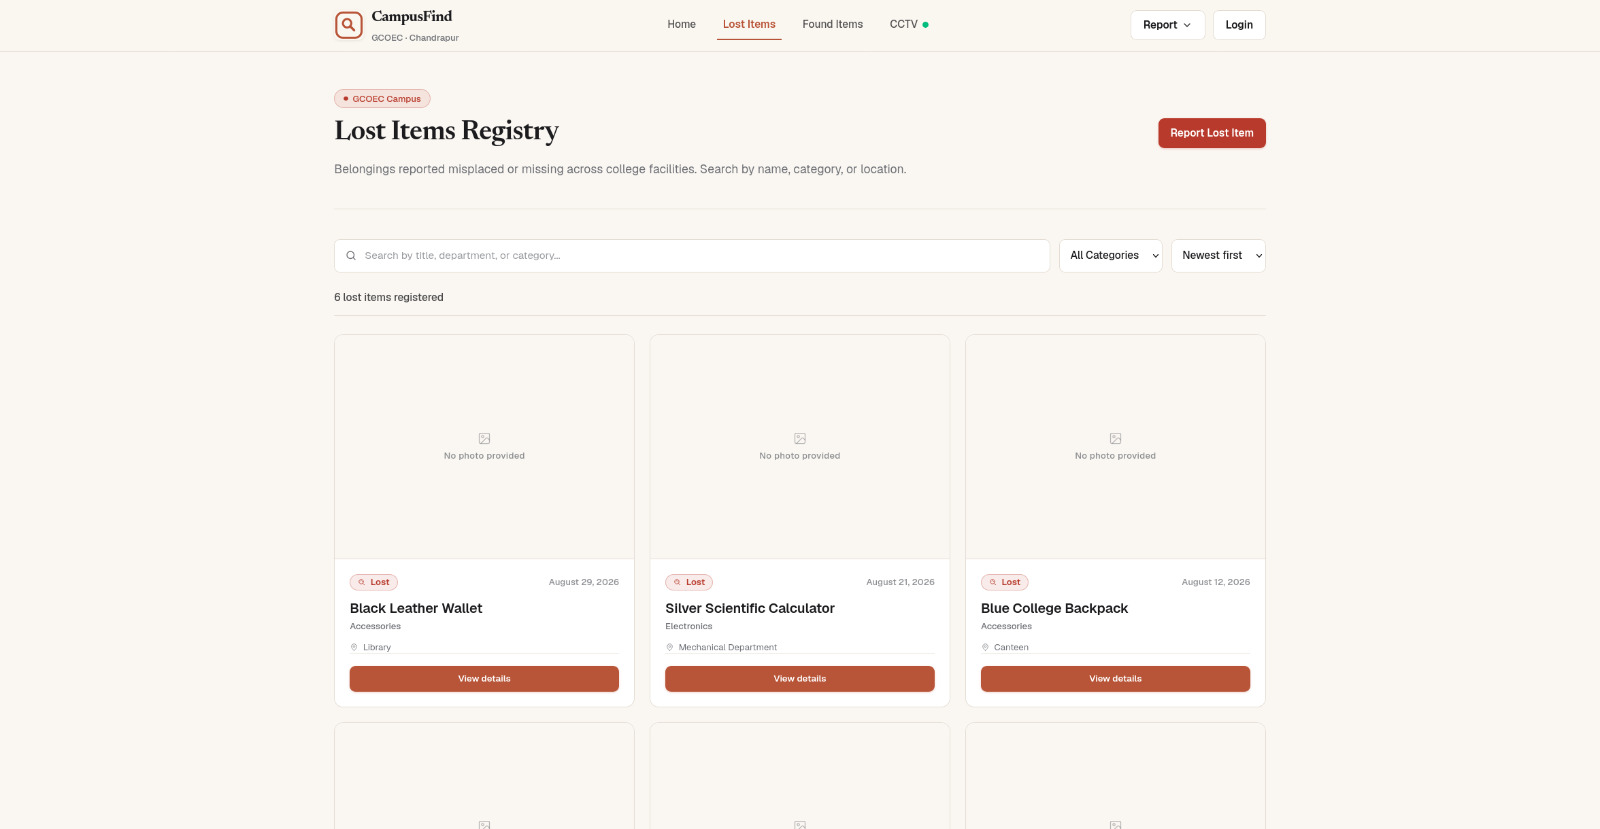
\includegraphics[width=0.92\textwidth]{IMGs/fig1_lost_registry.jpeg}
\caption{Lost Items Registry Interface (\texttt{/lost-items}) displaying real-time search, category filters, and protected card listings with generic vector archetypes.}
\end{figure}

\vspace{0.8cm}

\begin{figure}[H]
\centering
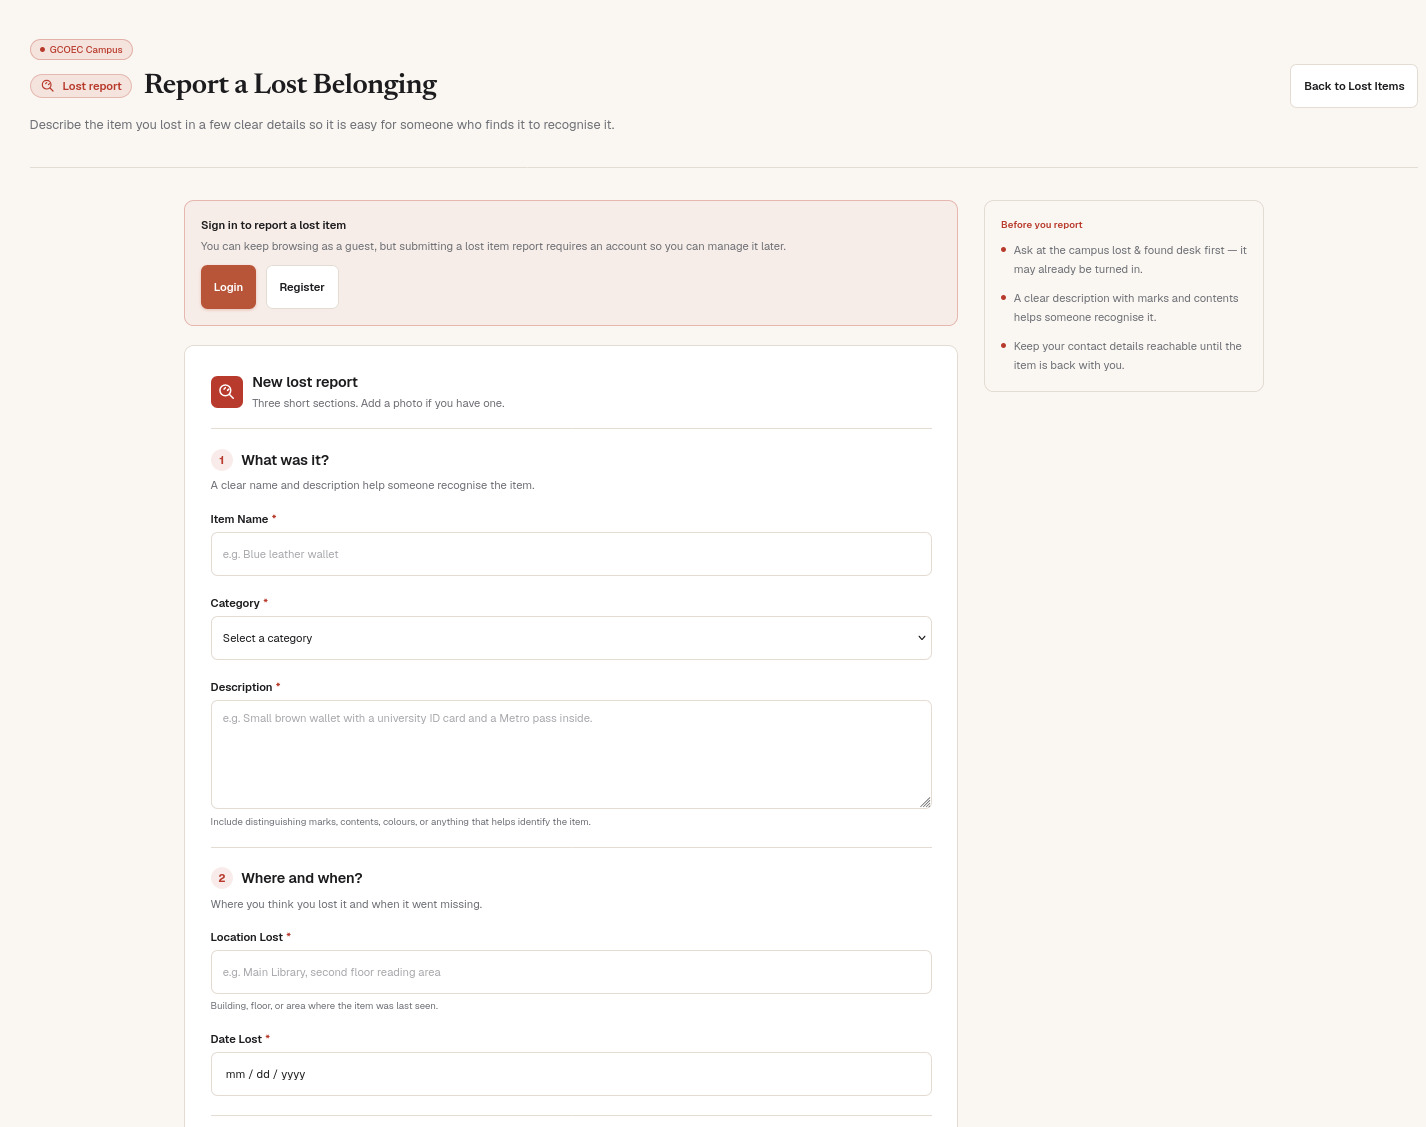
\includegraphics[width=0.92\textwidth]{IMGs/fig2_report_lost.jpeg}
\caption{Report a Lost Belonging Form (\texttt{/report-lost}) incorporating mandatory attribute validation, location tagging, date pickers, and security guidance.}
\end{figure}

\newpage

\begin{figure}[H]
\centering
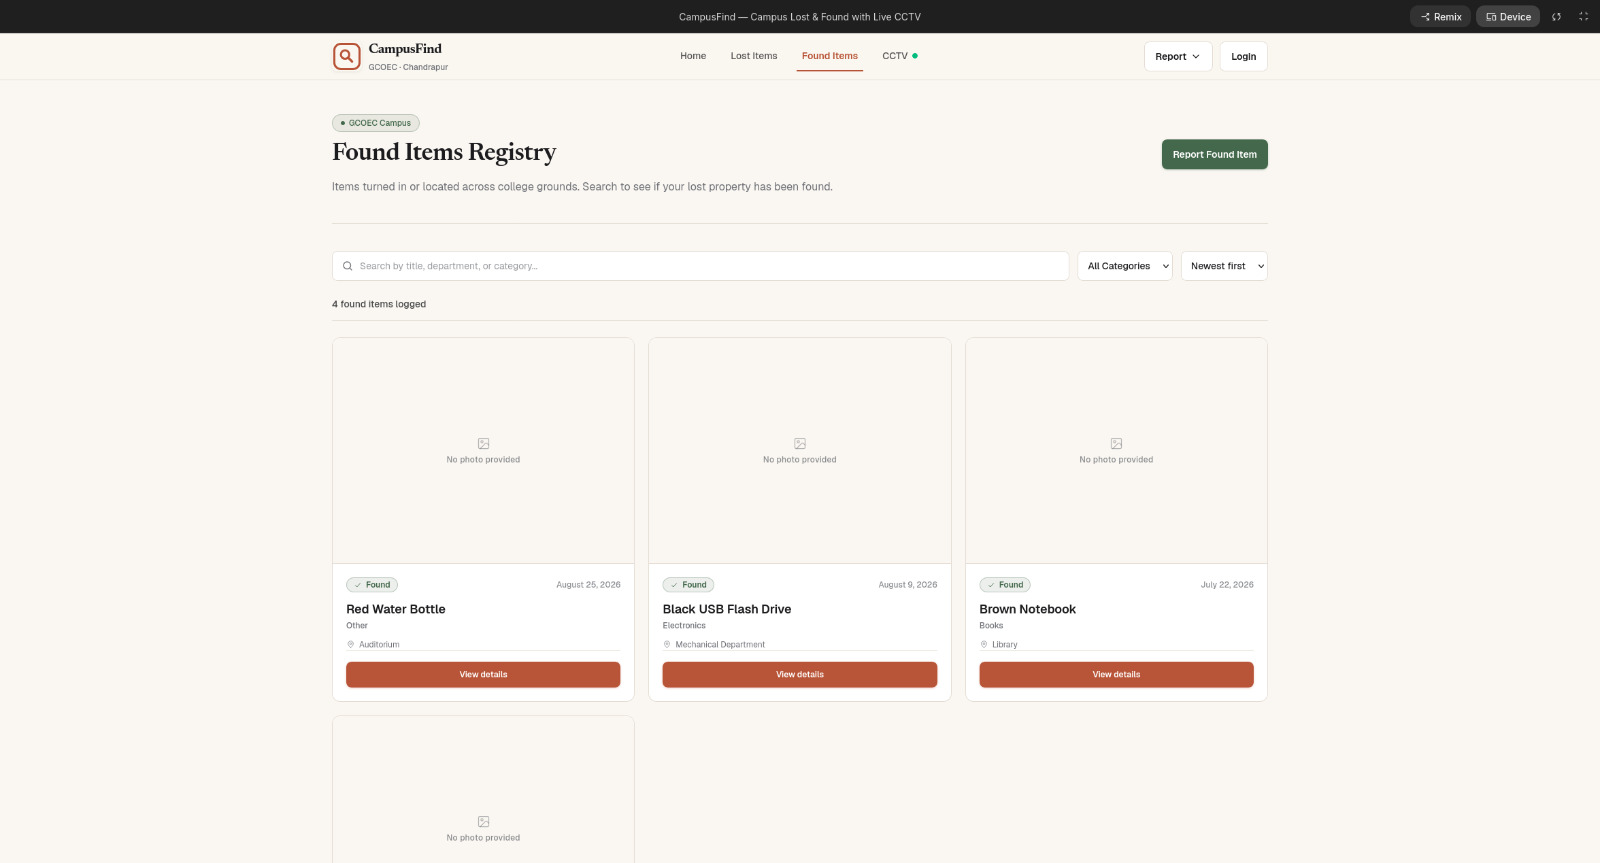
\includegraphics[width=0.92\textwidth]{IMGs/fig3_found_registry.jpeg}
\caption{Found Items Registry Interface (\texttt{/found-items}) cataloguing turned-in property across campus departments and laboratories.}
\end{figure}

\vspace{0.8cm}

\begin{figure}[H]
\centering
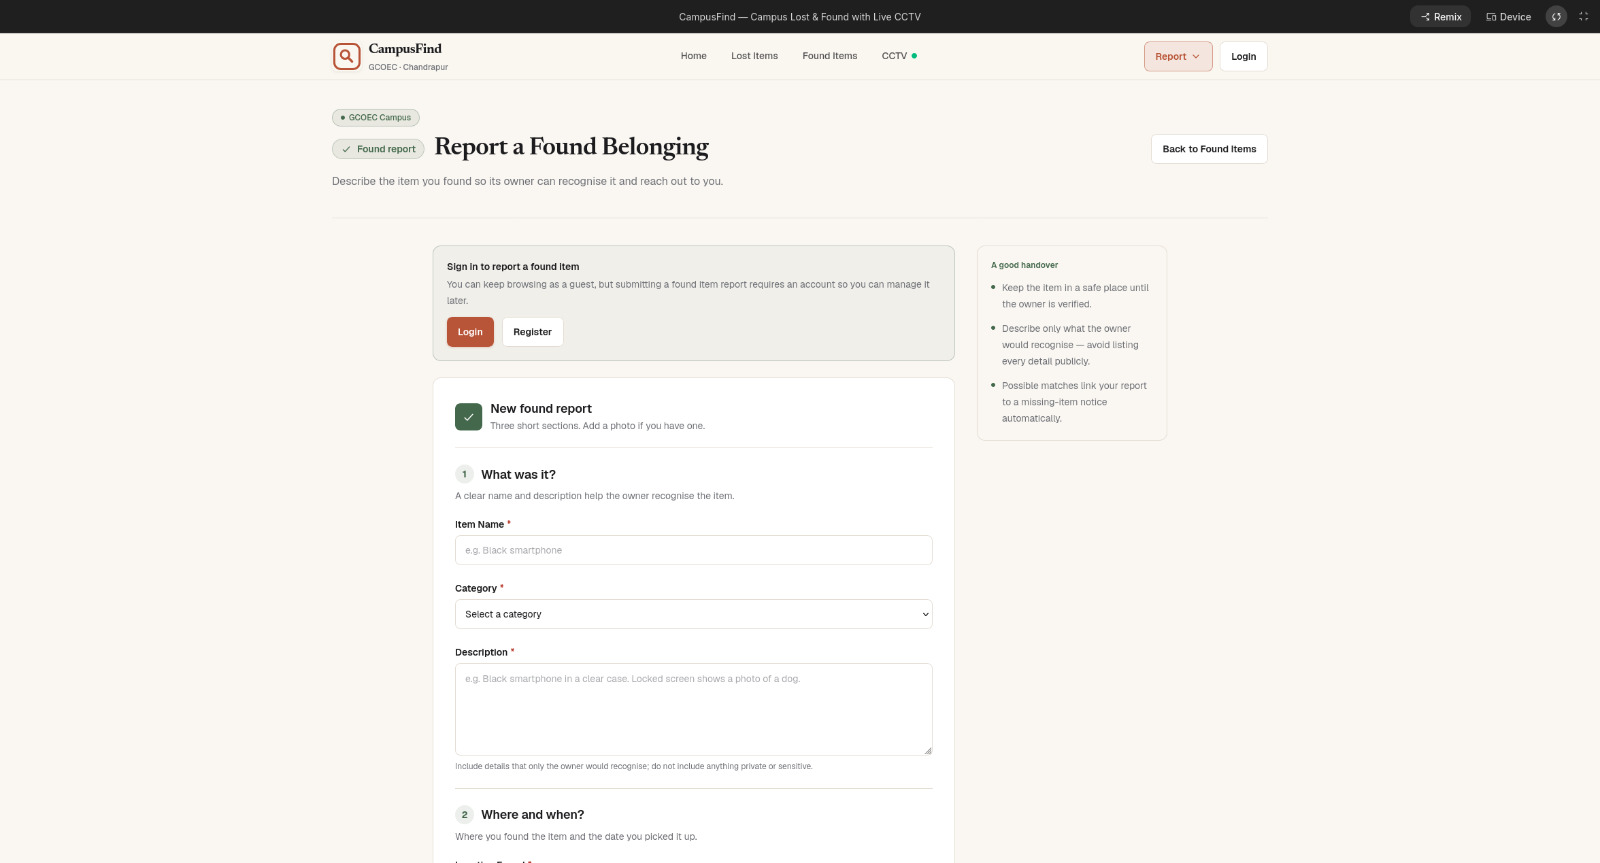
\includegraphics[width=0.92\textwidth]{IMGs/fig4_report_found.jpeg}
\caption{Report a Found Belonging Form (\texttt{/report-found}) facilitating the logging of discovered property with safe custody guidance.}
\end{figure}

\newpage

\begin{figure}[H]
\centering
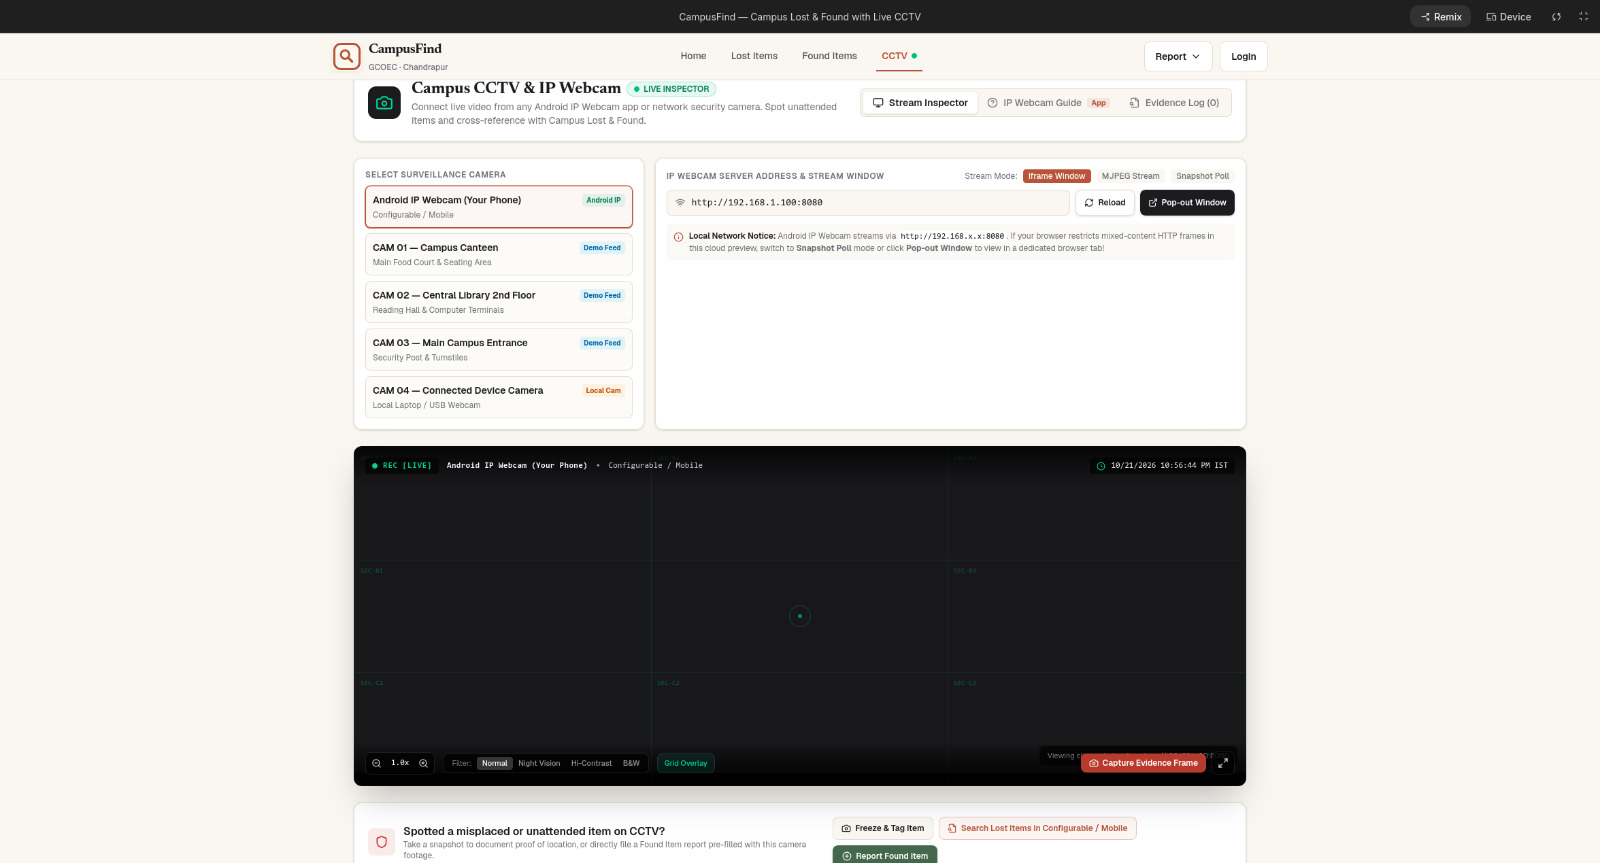
\includegraphics[width=0.92\textwidth]{IMGs/fig5_cctv_console.jpeg}
\caption{Campus CCTV \& IP Webcam Inspection Console (\texttt{/cctv}) featuring real-time stream feeds, camera switcher, inspection HUD, grid overlay, and evidence frame capture actions.}
\end{figure}

\vspace{0.8cm}

\begin{figure}[H]
\centering
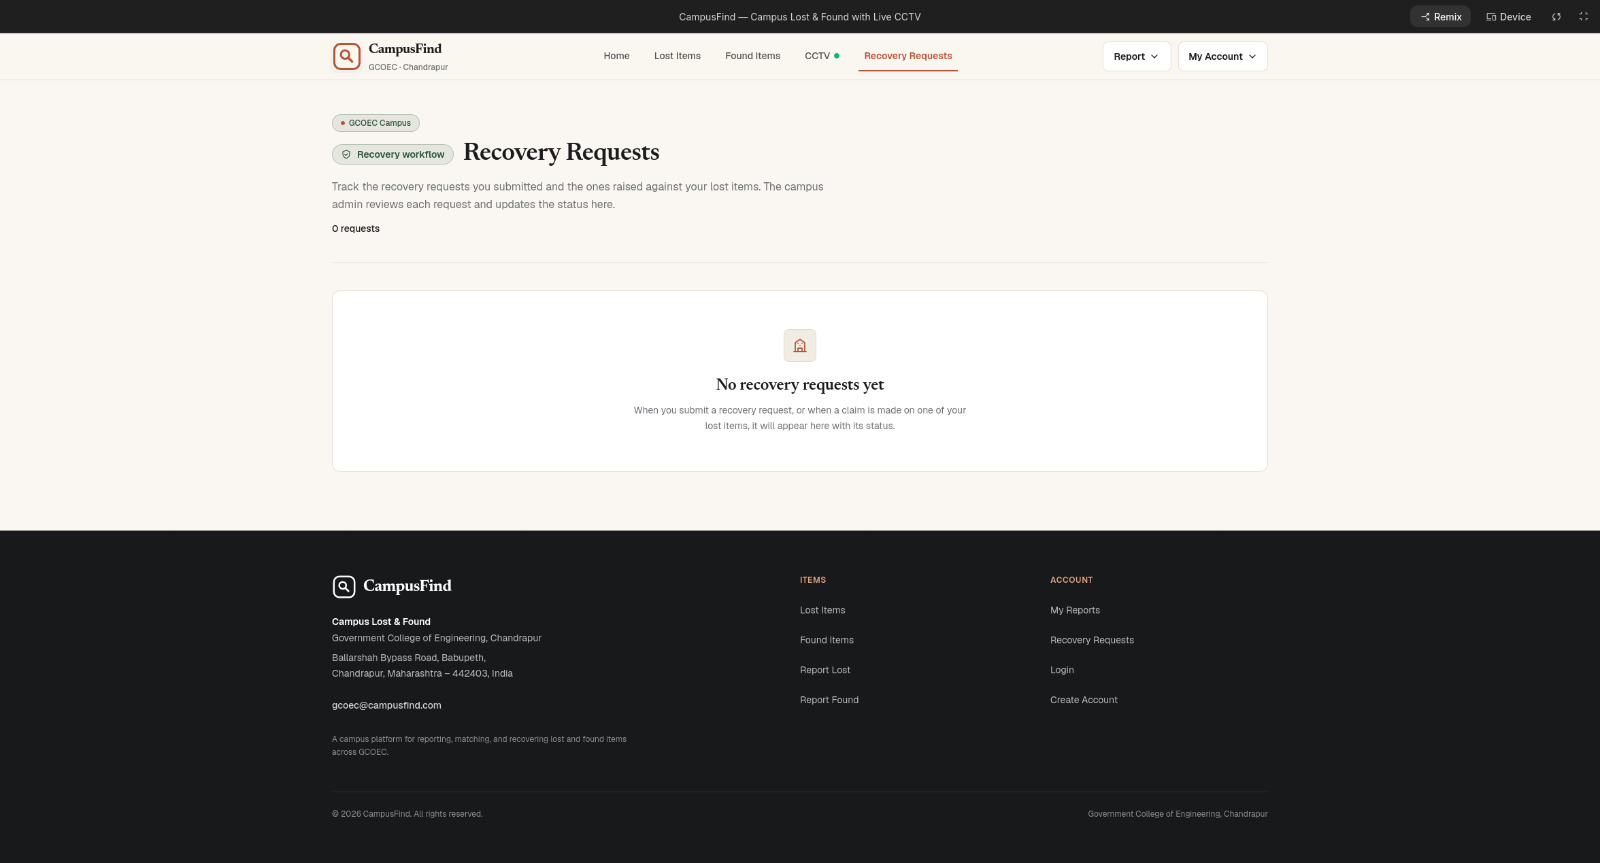
\includegraphics[width=0.92\textwidth]{IMGs/fig6_recovery_requests.jpeg}
\caption{Recovery Requests Workflow Management (\texttt{/recovery-requests}) where ownership claims are tracked, verified, and moderated by campus administration.}
\end{figure}

\newpage

\begin{figure}[H]
\centering
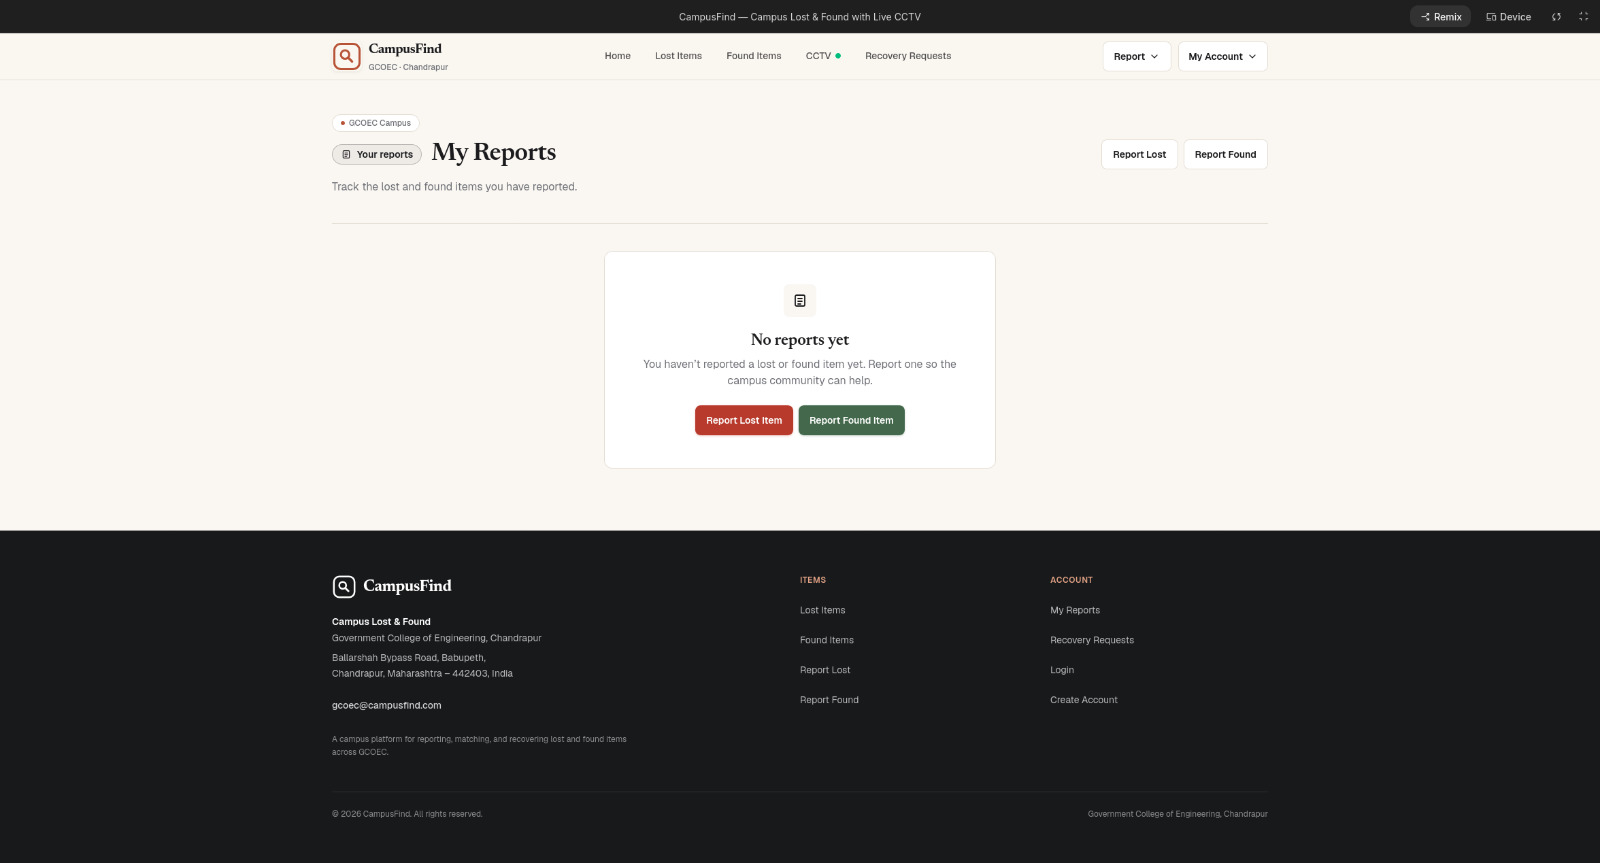
\includegraphics[width=0.92\textwidth]{IMGs/fig7_my_reports.jpeg}
\caption{User Activity and Reports Dashboard (\texttt{/my-reports}) providing authenticated students and faculty with an overview of their submitted listings.}
\end{figure}

\end{document}
